\documentclass[a4paper,12pt]{article}
\usepackage{amsmath, amsthm, amsfonts, amssymb}
\usepackage{mathtools}
\usepackage{microtype}
\usepackage{geometry}
\usepackage{booktabs}
\usepackage{graphicx}
\usepackage{tikz}
\usetikzlibrary{calc}

\newcommand*\diff{\mathop{}\!\mathrm{d}}

\usepackage{caption}
\usepackage{subcaption}
% \geometry{margin=1in}

\usepackage{enumitem}

\usepackage{hyperref}
\usepackage{xcolor}
\hypersetup{ % this is just my personal choice, feel free to change things
    colorlinks,
    linkcolor={red!50!black},
    citecolor={blue!50!black},
    urlcolor={blue!80!black},
}
\usepackage[capitalise]{cleveref}

\usepackage[T1]{fontenc}
\usepackage{sectsty}

\sectionfont{\scshape\mdseries\large}
\subsectionfont{\centering\scshape\bfseries\normalsize}
\numberwithin{equation}{section}

\colorlet{myred}{red!20}
\colorlet{myblue}{blue!20}
\colorlet{mypurple}{purple!40}
\colorlet{myorange}{orange!20}
\colorlet{myteal}{teal!35}

\DeclarePairedDelimiter\abs{\lvert}{\rvert}%
\DeclarePairedDelimiter\norm{\lVert}{\rVert}%

\newtheorem{theorem}{Theorem}

\title{
    MEK4250\\
    \small{Exam preperation for Finite Elements in Computational Mechanics}
}
\author{August Femtehjell}
\date{Spring 2025}

\begin{document}

\maketitle

\tableofcontents

\begin{abstract}
    This document contains my preperation for the final oral exam for the course MEK4250--Finite Elements in Computational Mechanics, taught at the University of Oslo in the spring of 2025.
    The code for everything, as well as this document, can be found at my GitHub repository: \url{https://github.com/augustfe/MEK4250}.
\end{abstract}

\section*{Exam formalities}
Six problems/topics are given for this exam.
For each problem, the candidate must prepare a 20 minutes oral presentation.
Try to communicate a good overview and understanding of the topic, but compose the talk so that you can demonstrate knowledge about details too.
The student is expected to be able to stick to one subject for the 30 minutes for top grades.
There are no aids besides a whiteboard and this document with the exam problems (experience with this type of exam and various aids tells that learning the content by heart gives by far the best delivery that demonstrates solid understanding).

We will throw a die and the number of eyes determines the topic to be presented.
After your presentation, you will be given some questions, either about parts of your presentation or facts from the other topics.
After each presentation, the next candidate can throw the die and thereby get about 10 minutes to collect the thoughts before presenting the assigned topic.


\section{The finite element method}
Explain Ciarlet's definition of a finite element.
Explain the concept of functionals and function spaces.
How are degrees of freedom used to ensure that the finite element spaces are part of certain function spcaes?
Show that a finite element may conveniently be defined in terms of a reference element.
List common elements in common spaces.

\subsection{Short-form answer}
\subsubsection{Ciarlet's definition}
Ciarlet defined a finite element as a triplet $(T, V, D)$.
Here, $T$ is a bounded domain in $\mathbb{R}^d$, which is typically a polyhedron.
This corresponds to a section of the triangulation of the domain.
Next, $V = \{\psi_i\}_{i = 1}^n$ is a set of linearly independent basis functions defined on $T$.
Finally, $D = \{d_i\}_{i = 1}^n$ is a set of degrees of freedom, which are linear functionals defined on $V$.

We typically want each domain $T$ to be shape regular, i.e.\ such that they are all triangles or all quadrilaterals.
This allows us to perform the computations in a more efficient manner, where we are able to reuse a lot of the computations for each element.
Note that the basis functions $\psi_i$ are only defined locally on the element $T$, and thus they are not defined globally.

The degrees of freedom $d_i$ are what tie the local basis functions together, ensuring properties such as continuity of a certain order across the boundaries of the elements.
With the degrees of freedom, we have the associated \textit{nodal basis} $\{\phi_{i}\}_{i = 1}^n$, which are defined such that
\begin{equation}
    d_j(\phi_i) = \delta_{ij}.
\end{equation}
Finite elements are typically implemented directly through this nodal basis, where the coefficients of the basis functions are defined by the degrees of freedom.

\subsubsection{Functionals and function spaces}
Function spaces are vector spaces, where each element is a function.
Typically, we are looking at function spaces defined through various properties, such as the space of all continuous functions, or the space of all functions with a finite integral.
A functional on a vector space $V$ is then an object $L(\cdot)$, which takes in a vector $v \in V$ and returns a number.
For instance, from a set of coordinates $x_1, x_2, \ldots, x_n$, we can define a functional $L$ on a function space $V = \Span\{\phi_i\}_{i=1}^n$ such that
\begin{equation}
    L(v) = v(x_1) + v(x_2) + \cdots + v(x_n),
    \qquad
    v \in V
\end{equation}
or a set of functionals $L_j$ such that
\begin{equation}
    L_j(\phi_i) = \phi_i(x_j) = \delta_{ij},
    \qquad
    i = 1, 2, \ldots, n.
\end{equation}

Typical function spaces we are interested in the finite element method are Sobolev spaces $W^{k,p}(\Omega)$, which are defined as
\begin{equation}
    W^{k,p}(\Omega) =
    \left\{
        u :
        \left(
            \int_{\Omega}
            \sum_{i \leq k} \abs*{\frac{\partial^i u}{\partial x^i}}^p
            \diff x
        \right)^{1/p} < \infty
    \right\},
\end{equation}
essentially spaces where the function and its derivatives up to order $k$ are in $L^p(\Omega)$.

As far as I'm aware, we are really only interested in the spaces where $p = 2$, which we denote as $H^k(\Omega)$.
The $H$ is chosen after Hilbert, as these are in fact Hilbert spaces.
The inner product for $H^k(\Omega)$ is defined as
\begin{equation}
    (u, v)_{H^k(\Omega)}
    = (u, v)_k
    = \sum_{i \leq k} \int_{\Omega} \frac{\partial^i u}{\partial x^i} \frac{\partial^i v}{\partial x^i} \diff x.
\end{equation}
With the functionals we defined previously, if we choose the points $x_i$ to be along the edges of the elements, we can ensure that they are continuous across elements, which then gives us that the finite element space is a subspace of $H^1(\Omega)$.
Similarly, we can choose a different set of functionals such that we ensure higher order continuity, such as $H^2(\Omega)$.

\subsubsection{Reference element}
In order to illustrate the benefit of a reference element, we consider simply a number of segments of the real number line, with points $x_1 < x_2 < \cdots < x_n$.
Thus, each $T_i$ is simply the segment $[x_i, x_{i+1}]$ for $i = 1, 2, \ldots, n-1$.
On each segment, we have the linear Lagrange basis functions $\phi_i$, which are defined such that $\phi_i(x_j) = \delta_{ij}$.
This is illustrated with $n = 5$ points in \cref{fig:segments}.

\begin{figure}[htbp]
    \centering
    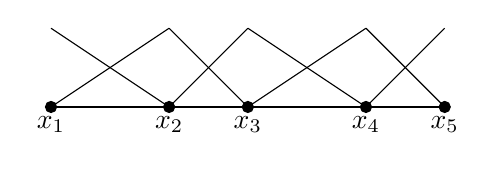
\begin{tikzpicture}
        \def\N{4} % Number of segments
        \foreach \x/\i in {0/1, 1.5/2, 2.5/3, 4/4, 5/5} {
            % Draw a filled circle of radius 2pt at (\x,0) and name that coordinate (x\i)
            \draw[fill=black] (\x,0) circle (2pt) coordinate (x\i);

            % Place the label "x_i" just below the same point (x\i)
            \node[below] at (x\i) {$x_{\i}$};
        }
        \draw[thick] (x1) -- (x\the\numexpr\N + 1\relax);

        \foreach \i in {1,...,\the\numexpr\N\relax} {
            \draw ($(x\i)+(0,1)$) -- (x\the\numexpr\i+1\relax);
            \draw (x\i) -- ($(x\the\numexpr\i+1\relax)+(0,1)$);
        }
    \end{tikzpicture}
    \caption{A number of segments of the real number line, with points $x_1 < x_2 < \cdots < x_n$, defining basis functions $\phi_i$ on each segment.\label{fig:segments}}
\end{figure}

When solving the finite element problem, we typically need to compute matrices $A$ and $M$ defined by
\begin{equation}
    A_{ij} = \int_{\Omega} \nabla \phi_i \cdot \nabla \phi_j \diff x,
    \qquad
    M_{ij} = \int_{\Omega} \phi_i \phi_j \diff x,
\end{equation}
where $A$ is the stiffness matrix and $M$ is the mass matrix.
With the basis functions we have here, these matrices will be incredibly sparse, as for instance $\phi_i$ is only non-zero on the segment $[x_{i-1}, x_{i+1}]$.
As such, we can beforehand say that for instance $A_{1,5}$ will be zero.

We then only need to compute the integrals for the non-zero entries, and we can additionally do this just on each segment, rather than the entire domain.
We are then left with the integrals of the form
\begin{equation}
    A_{ij}
    = \int_\Omega \phi'_i(x) \phi'_j(x) \diff x
    = \int_{x_i}^{x_{i+1}} \phi'_i(x) \phi'_j(x) \diff x
\end{equation}
for $j = i, i+1$.
As of now, we need to compute this for each $i$, however with a change of basis we can instead compute it just once for each segment, getting
\begin{equation}
    A_{j, k}^{(i)} = \int_{0}^{1} \ell'_j(X) \frac{\diff X}{\diff x} \ell'_k(X) \frac{\diff X}{\diff x} \frac{\diff x}{\diff X} \diff X,
\end{equation}
where $X$ is the reference element, and $dX/dx$ is the Jacobian of the transformation from the reference element to the segment.
In the linear case, $\frac{dX}{dx}$ is simply the length of the segment, and we can pull it out of the integral.
Constructing the total stiffness matrix then becomes a matter of computing the integral once for the reference element, and then adding the scaled contributions for each segment.
A similar argument holds for higher order spaces, mapping the physical element to the reference element, however the Jacobian will be more complicated, especially in the case of curved elements.

\subsubsection{Common elements in common spaces}
As mentioned previously, we are mostly interested in the spaces $L^2$, $H^1$ and $H^2$, as well as the spaces $H(\mathrm{div})$ and $H(\mathrm{curl})$.
Let's firstly describe the new spaces $H(\mathrm{div})$ and $H(\mathrm{curl})$.
They are given by
\begin{equation}
    \begin{split}
        H(\mathrm{div}) &= \left\{ u \in L^2(\Omega)^d : \nabla \cdot u \in L^2(\Omega) \right\},\\
        H(\mathrm{curl}) &= \left\{ u \in L^2(\Omega)^d : \nabla \times u \in L^2(\Omega) \right\}.
    \end{split}
\end{equation}

We are typically working with polynomial spaces, which are $C^\infty$ within their domain.
If we allow for discontinuities across the boundaries, we are in $L^2$.
If we enforce continuity across the boundaries, we are in $H^1$, and are typically using Lagrange elements.
If we enforce continuity of the first derivatives as well, we are in $H^2$, and are typically using Hermite elements.
For the spaces $H(\mathrm{div})$ and $H(\mathrm{curl})$, we typically use Raviart-Thomas elements and Nedelec elements respectively.

Raviart-Thomas elements ensure continuity of the normal component across boundaries, while jumps in the tangential component are allowed.
Similarly, as Stokes' Theorem relates curl to the tangential component, Nedelec elements ensure continuity of the tangential component across boundaries, while jumps in the normal component are allowed.

\subsection{Long-form answer}

\subsubsection{Ciarlet's definition of a finite element}
Ciarlet defines a finite element by a triplet $(T, V , D)$, where
\begin{itemize}
    \item
        $T$ is a bounded domain in $R^d$, most typically a polyhedron.

    \item
        $V = \{\psi_i\}_{i = 1}^n$ is a set of linearly independent basis functions on $T$

    \item
        $D = \{d_i\}_{i = 1}^n$ is a set of (linearly independent) degrees of freedom defined in terms of linear functionals on $V$.
        (We remark for $v \in V$ we may evaluate $d_i(v)$ since $d_i$ is a linear functional on $V$.)
\end{itemize}
$T$ defines the triangulation, or cells, in our domain.
The basis functions are then just defined on their cell $T$.
The magic happens when we introduce $D$, dubbed the degrees of freedom, or dofs for short.
They are in a sense how we ``tie'' the function spaces together, as they are originally just defined locally.

Most elements are implemented through a nodal basis, defined by the set of basis functions $\{\phi_i\}_{i = 0}^n$ satsifying $d_j(\phi_i) = \delta_{ij}$.
The simplest example is the Lagrange element, where for a basis function $L_j$, the dofs are defined by
\begin{equation}
    d_i(L_j) = L_j(x_i) = \delta_{ij}.
\end{equation}
Initially, the set $\{x_i\}$ consists of the nodes of each triangle.

Say we have two triangles, each with the vertices $\{x_1, x_2, x_3\}$ and $\{x_4, x_5, x_6\}$ respectively.
If the triangles are next to eachother, we would perhaps then have that $x_2 = x_4$ and $x_3 = x_5$.
However, we still av the set of dofs $\{d_i\}_{i = 1}^{6}$, even though we only have four unique points.
This results in discontinuous Lagrange elements, as they do not directly communicate across the boundaries.
If we however say that $d_2 = d_4$ and $d_3 = d_5$, we would have continuous elements.

\subsubsection{Concept of functionals and function spaces}
A function space is a vector space where each element is a function.
Typically, the function spaces are defined by some properties, for instance the space of all continuous functions, all functions with a finite integral, and especially in our case all functions where the function as well as the derivatives have finite integrals.
This essentially forms our ``main'' space $H^1(\Omega)$, defined by
\begin{equation}
    H^1(\Omega) =
    \left\{
        f
        :
        \int_{\Omega} \abs{f}^2 + \abs{\nabla f}^2 \diff x < \infty
    \right\}.
\end{equation}
A functional is then simply something which takes in a vector, for instance from a function space, and returns a number, either real or complex (although typically real in our case).

\subsubsection{How DOFs define our space}


\end{document}